\documentclass[12pt]{article}
%\usepackage[left=1in, right=1in, top=0.5in, bottom=1in]{geometry}
\usepackage{amsmath}
\usepackage{graphicx}
\usepackage{xcolor}
\usepackage{enumitem}
\usepackage{setspace}
\usepackage{latexsym}
\usepackage{wasysym}
\usepackage{amssymb}
\usepackage{blindtext}
\usepackage{times}
\usepackage{float}
\usepackage{units}
\usepackage[top=2.5cm, bottom=2.5cm, left=2cm, right=2cm]{geometry}
\usepackage{fancyhdr}
\usepackage[bf]{caption}
\usepackage{pdfpages,caption}


\let\ds\displaystyle


\begin{document}


\title{ICS 675 / MBIO 740 - Short Project 1\\
DNA Sequencing Alignment on \textit{Prochlorococcus Marinus}}
\author{Mojtaba Abolfazli\\ Vincent Chung \\ Christopher Kang}
\date{February 28, 2020}
\maketitle

\newpage
\linespread{1.1}
\pagestyle{fancy}

\tableofcontents
\listoffigures

\newpage

\section{Introduction}
In this project, we further investigate whether the new protocols used in Illumina sequencing technology exhibit a bias by generating more reads in regions with enriched GC base pairs. We further investigate this claim by examining the bacteria Prochlorococcus Marinus, a type of bacteria that is found in the ocean. Its ubiquity and occurrence at high density from the surface down to the depths of 200m make it presumably the most abundant photosynthetic organism on Earth. Prochlorococcus Marinus therefore  plays a major role in the dynamics between organisms in the ocean by contributing a large amount to the photosynthetic production of oxygen. For such a small cyanobacteria to yield such a large biomass, this piqued our interest to further investigate the DNA sequence of the bacterium. In this project, we seek a conclusion to whether or not DNA sequencing generated by Illumina sequencing technology does in fact exhibit a bias towards GC rich regions.

\section{Methods}
\subsection{Data Collection}
From NCBI’s microbial genome page, we collected the complete genome of Prochlorococcus Marinus str. MIT 9313. Moving forward, we will utilize this complete genome as our reference. To find a short read to align back against the reference genome, we searched through SRA and used experiment ERX2194388 (published 2017). 

\subsection{Sequence Alignment}
To align the sequence back against the reference sequence, we utilized Bowtie 2 and BWA. The BWA-MEM algorithm was chosen to perform a local alignment, as it outperforms the BWA-backtrack algorithm for short Illumina reads. Briefly, the BWA-MEM algorithm claims to work by seeding alignments with maximal exact matches (MEMs) and then extending seeds with the affine-gap Smith-Waterman algorithm (SW). Formally, a maximal exact match is an exact match that cannot be extended in either direction, i.e. the alignment is trimmed until the alignment score is maximized.  A variety of parameters to control the accuracy and efficiency of the alignment were also available. For example, the flags -w, -k, -r, and -B, which control the bandwidth, minimum seed length, re-seeding, and mismatch penalty, respectively. The -r flag in particular was not set, as it supposedly decreases accuracy in exchange for faster alignment.  Just like the BWA-MEM algorithm, the Bowtie2 aligner can perform a local alignment, where it trims some read characters from one or both ends of the alignment if doing so maximizes the alignment score (maximal exact match). The Bowtie2 aligner has similar parameters to BWA such as seed spacing, seed length and the number of mismatches permitted. Additionally, both aligners have a paired-end mode.

\subsection{Sequence Alignment Visualization and Distribution Plots}
\begin{figure}
    \centering
    \includegraphics[width=1\textwidth]{Tablet_highGC.jpg}
    \caption{A screenshot using Tablet of a region with low GC content. Reads colored in red denote G or C base pairs, while reads colored in blue denote an A or T base pair read}
    \label{Figure 1}
    
    \includegraphics[width=1\textwidth]{Tablet_lowGC.jpg}
    \caption{A screenshot using Tablet of a region with high GC content. Reads colored in red denote G or C base pairs, while reads colored in blue denote an A or T base pair read}
    \label{Figure 2}
\end{figure}

\begin{figure}
    \centering
    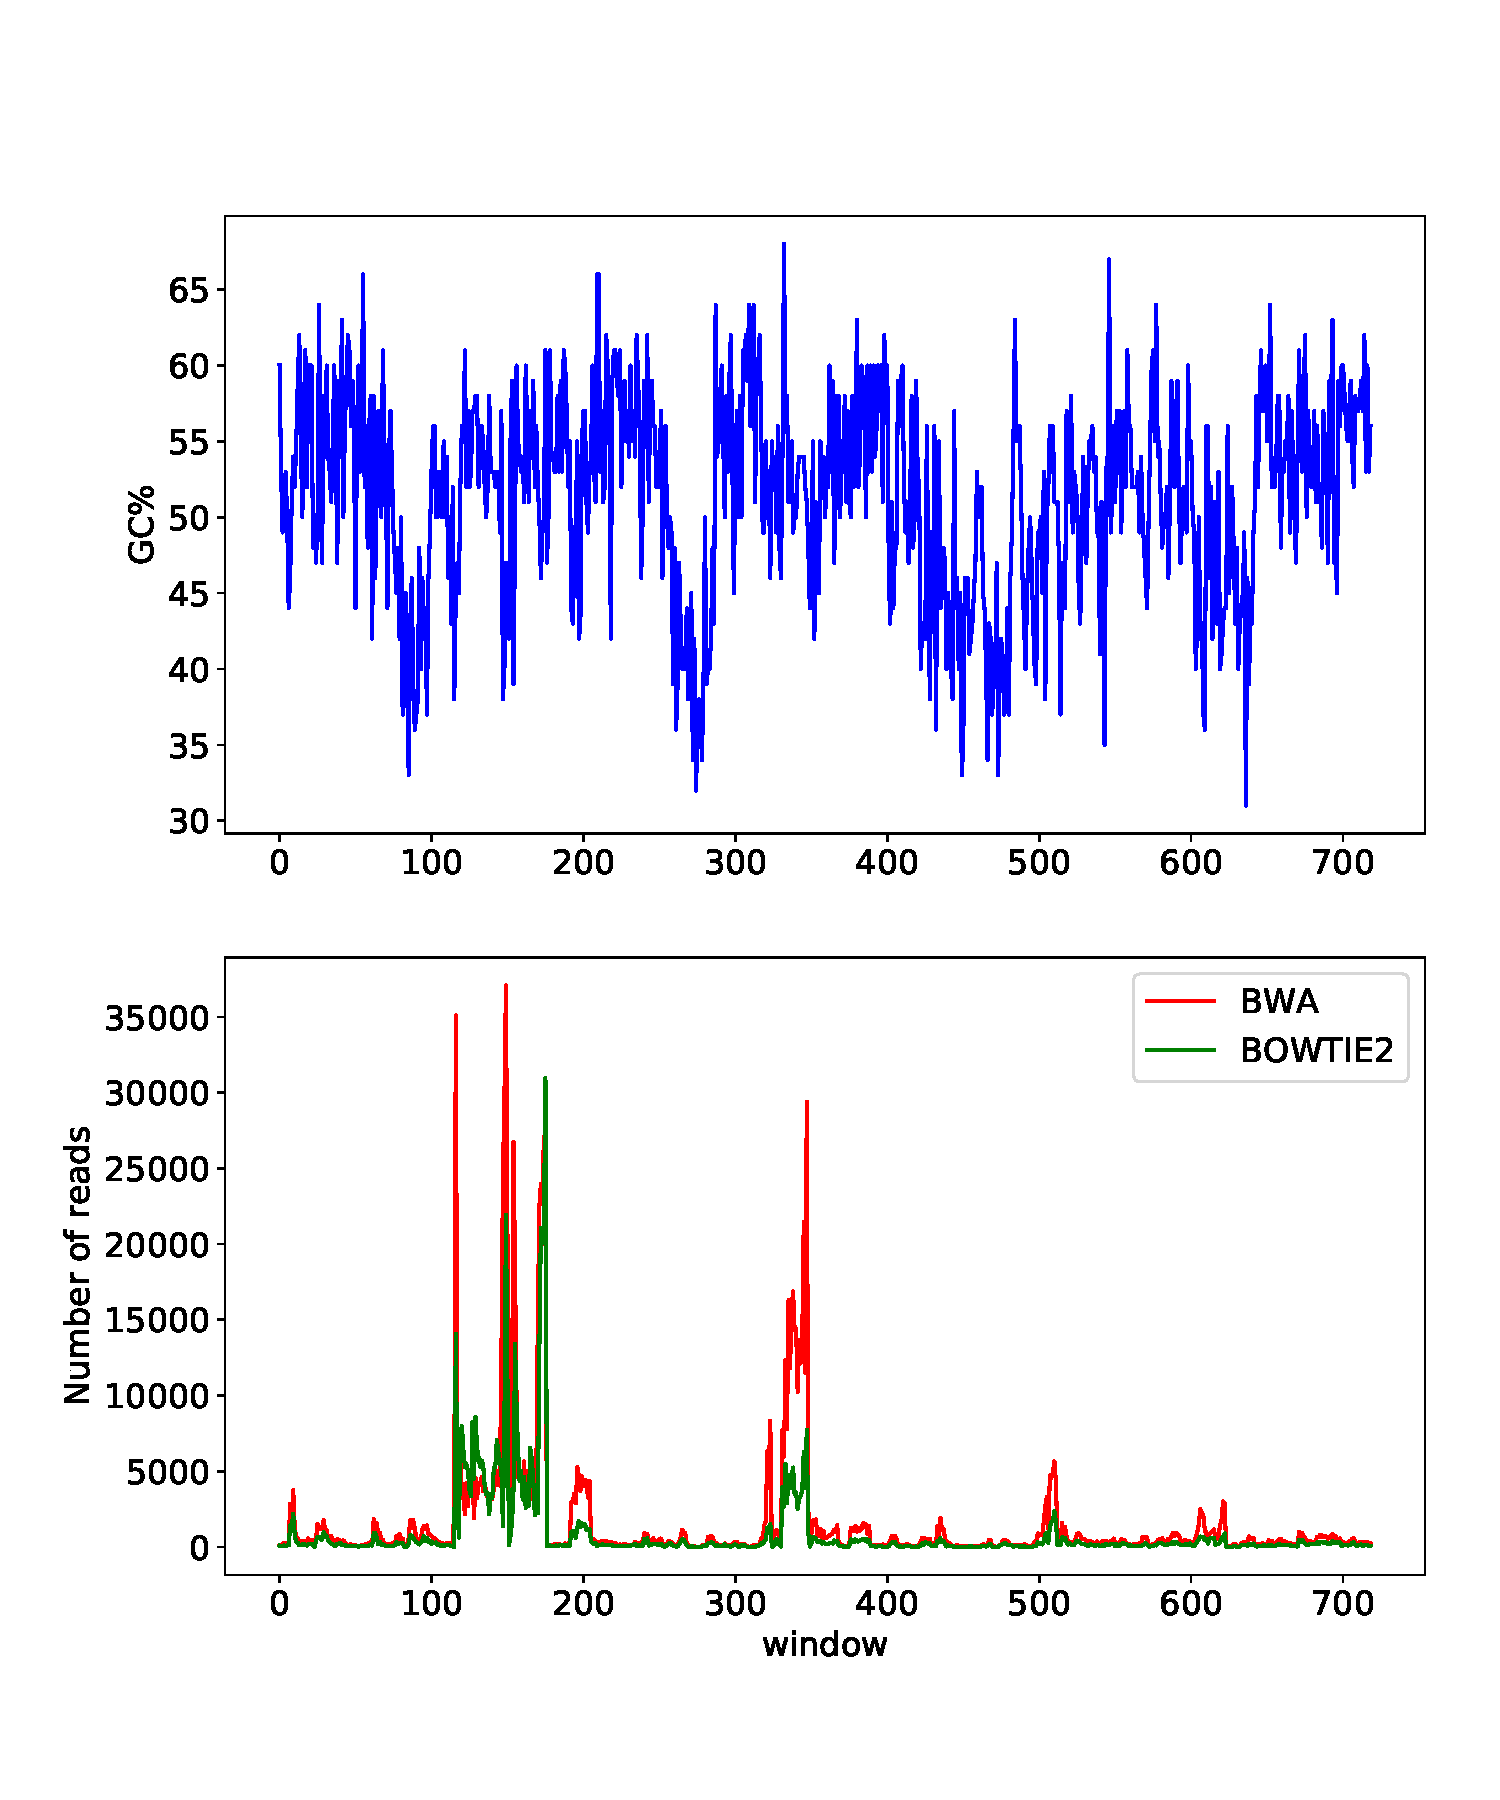
\includegraphics[width=1\textwidth]{Reads1.jpg}
    \caption{This graphic corresponds to the number of reads received as well as the GC\% of a region with high GC content (this corresponds to Figure 1)}
    \label{Figure 3}
\end{figure}

\begin{figure}
    \centering
    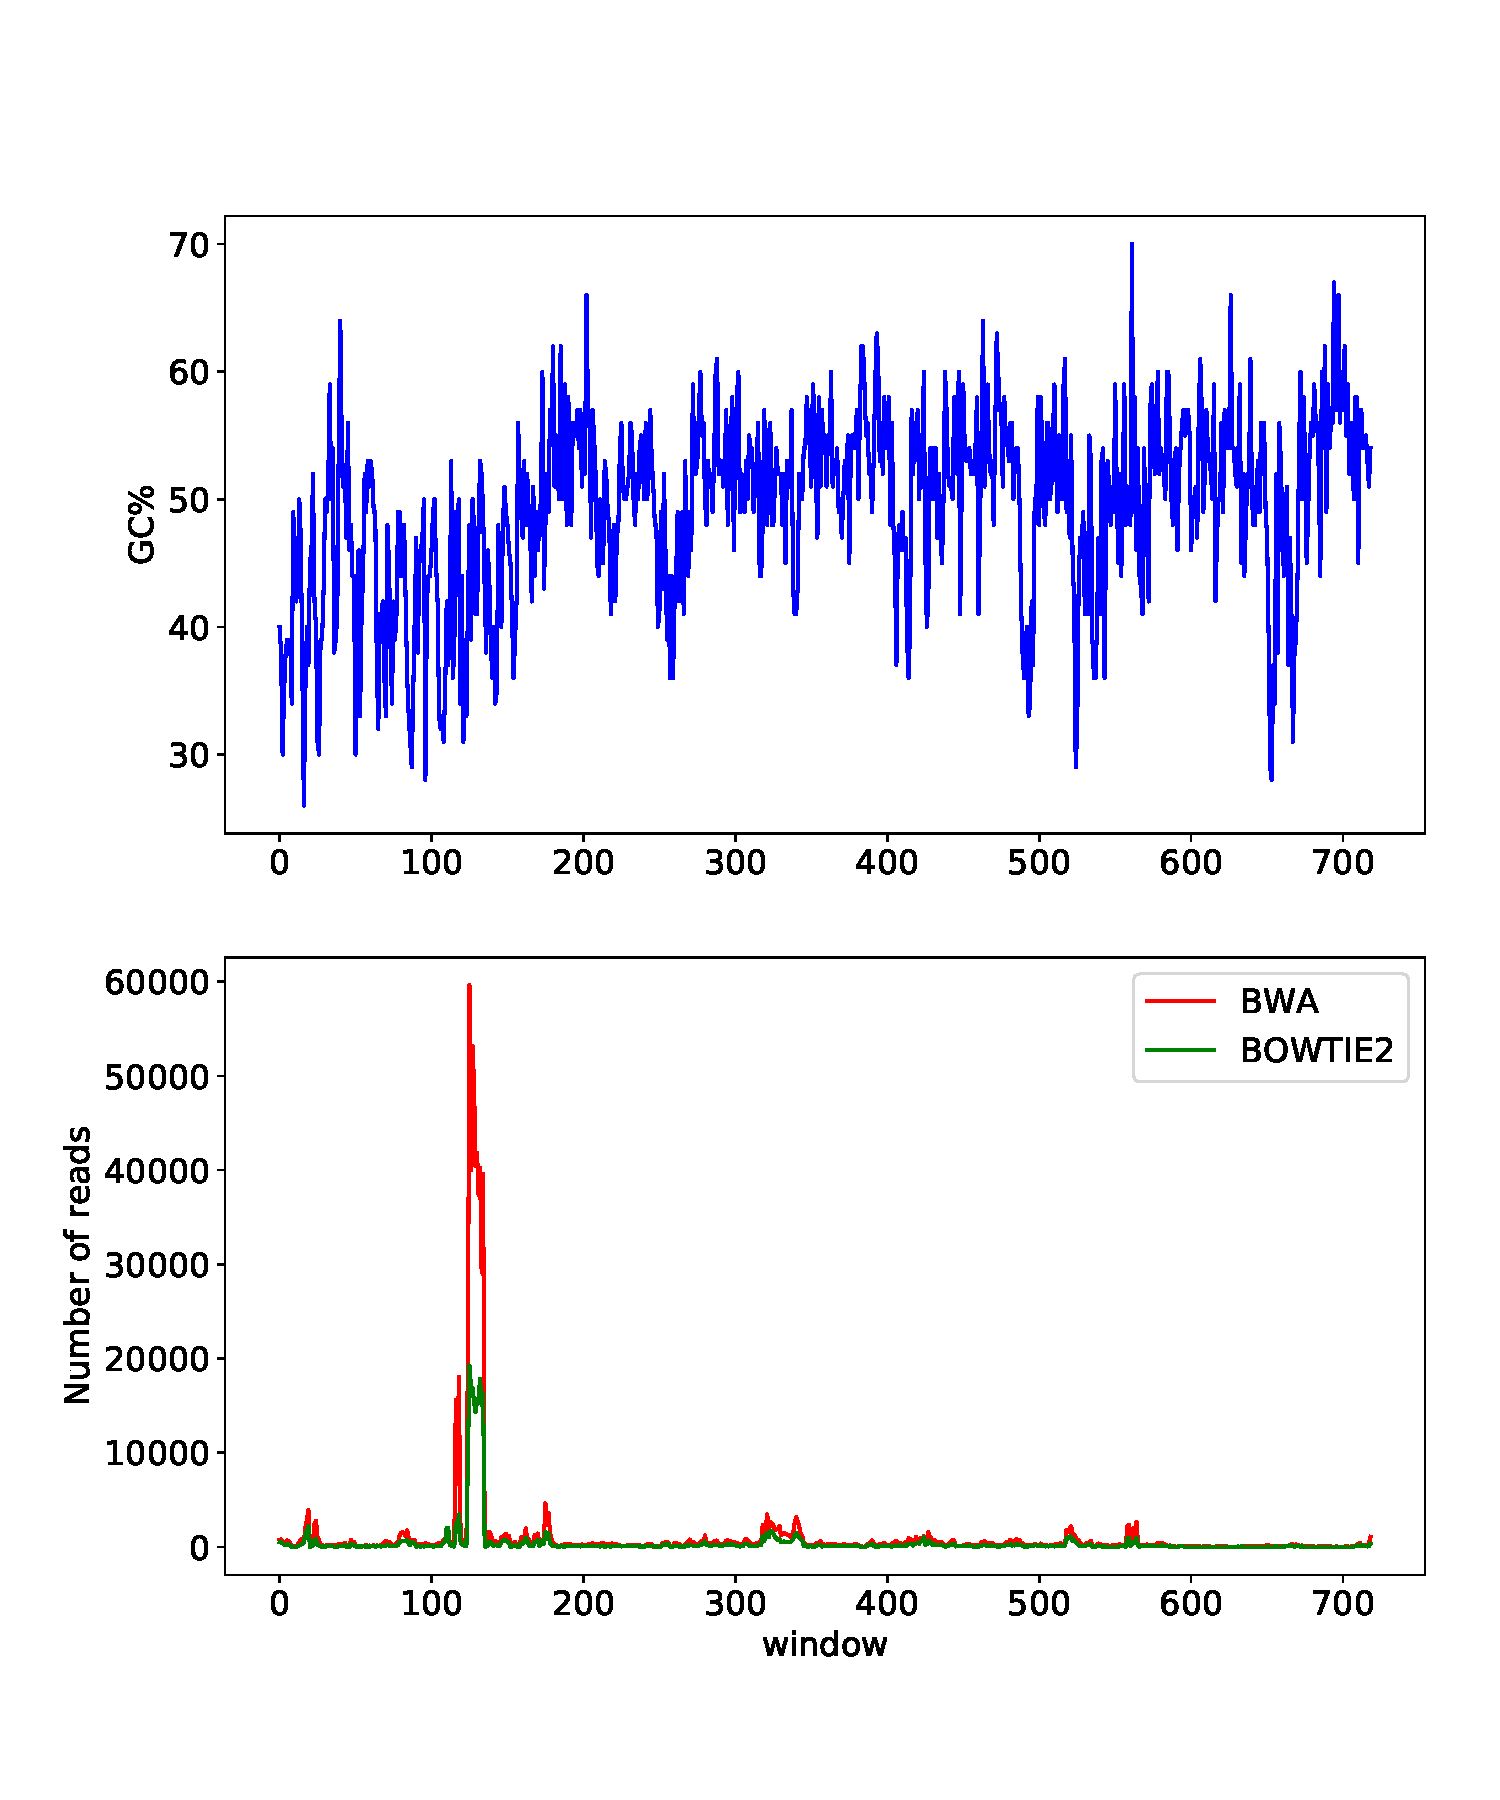
\includegraphics[width=1\textwidth]{Reads2.jpg}
    \caption{This graphic corresponds to the number of reads received as well as the GC\% of a region with low GC content (this corresponds to Figure 2)}
    \label{Figure 3}
\end{figure}


\begin{figure}
    \centering
    \includegraphics[width=1\textwidth]{GC_Histogram-page-001.jpg}
    \caption{A histogram plot that describes the GC\% and its associated probability}
    \label{Figure 3}

    \includegraphics[width=1\textwidth]{pdf_aligners-page-001.jpg}
    \caption{A plot that compares the reads between the two aligners of our choice: BWA and BOWTIE2}
    \label{Figure 4}
\end{figure}


%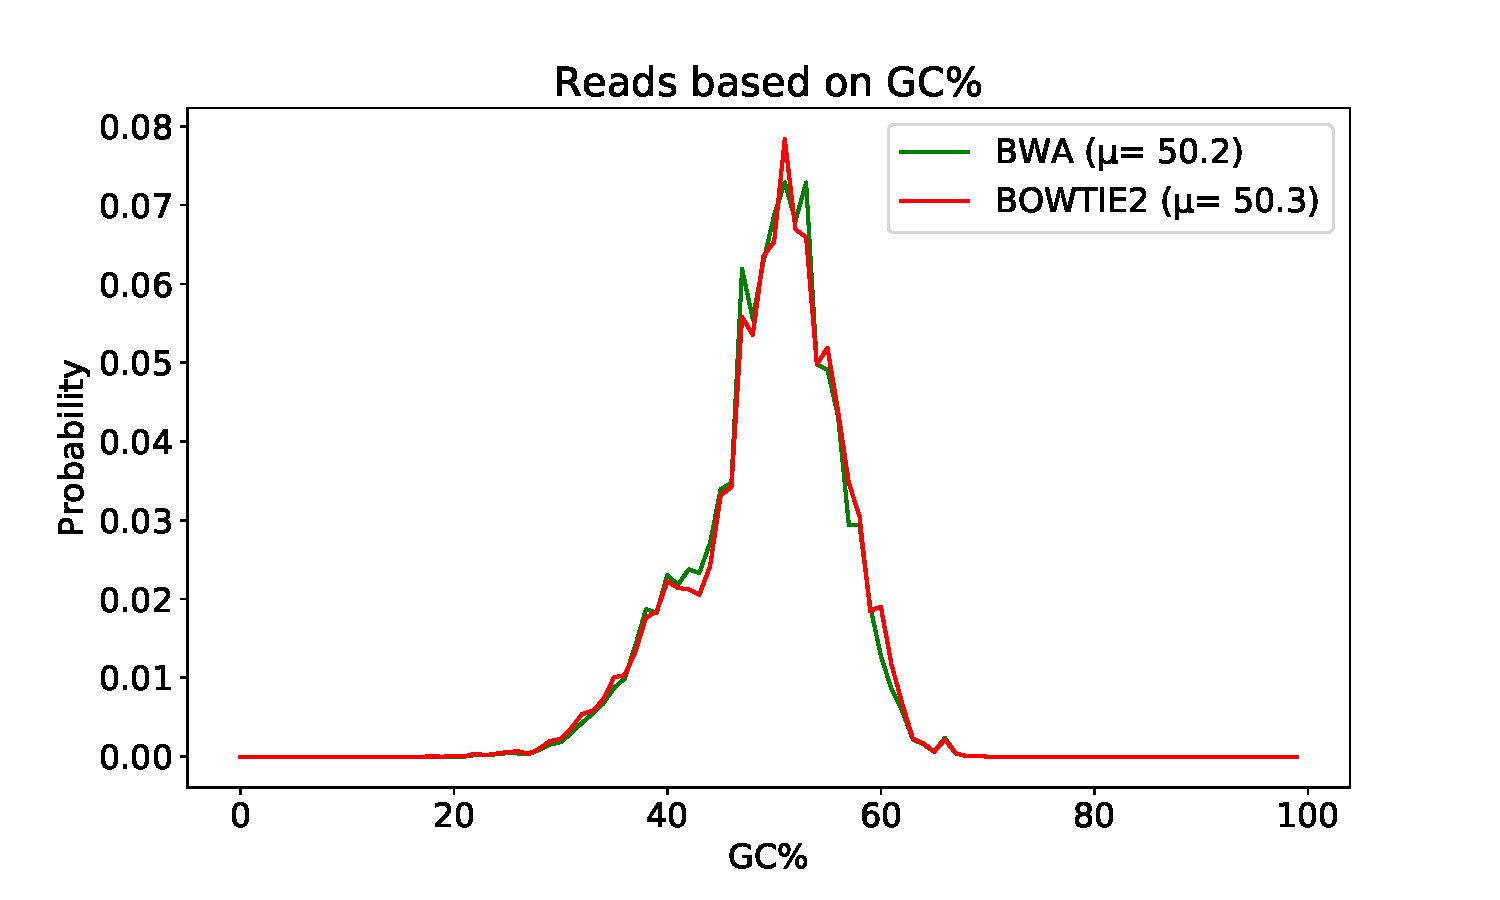
\includepdf[page={1}]{pdf_aligners.pdf}
%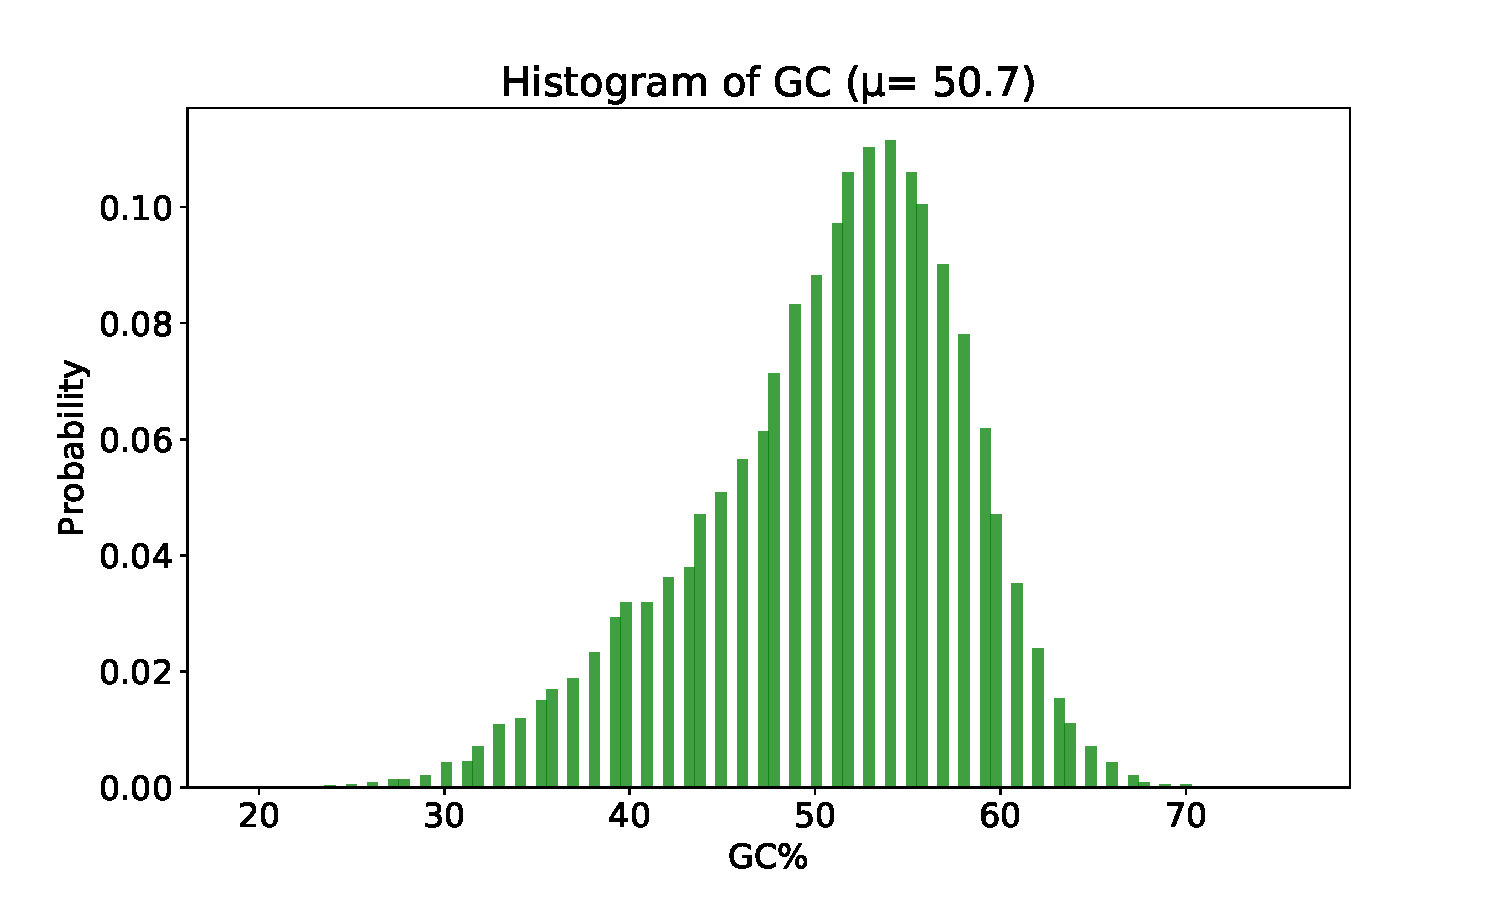
\includepdf[page={1}]{GC_Histogram.pdf}

\newpage

\section{Statistical Analysis of GC Concentration Regions}

\subsection{Motivation and Null Hypothesis}
{A 2008 study by Dohm et al. claims that short read data from high-throughput instruments gave a bias and generated certain regions with an enrichment in GC-base pairs. Therefore, the null hypothesis for this experiment is that the distribution of GC-base pairs will be overly represented, namely the distribution of GC-content will be significantly greater than $50\%$.}

\subsection{Development of Our Statistical Test}
{Upon looking at the distribution plot of the reads given by the aligners, the diagram suggests that the distribution of given from both reads resembles a standard normal distribution. Therefore, for this section, we employ a Z-test as our statistical test of choice to investigate the claim made in 2008 by Dohm et al. DNA sequencing is determined by four nucleotides: A, C, G, and T. Since we are interested in the GC-base pairs, theoretically, the distribution of the nucleotides should be about half AT-base pairs and the remaining half GC-base pairs. Consequently, we define the theoretical mean $\mu=0.5$. However, we decide to go against the claim of Dohm et al. and we suggest that GC-base pairs are not significantly over represented. Namely, we develop an alternative hypothesis that GC-content will not be significantly greater than $50\%$.}

\subsection{Analysis of Data}
{To further investigate this claim, we take a look at our data. According to our diagram which compares the reads between BWA and BOWTIE2, we found that the experimental average is determined to be $\hat{\mu_1}=50.2$ and $\hat{\mu_2}=50.3$, respectively. As we are using a Z-test, we employ the standard value of $\alpha = 0.05$. This implies we have a critical value of $z_{0.05}=1.645$. Our goal is to determine whether or not $Z\geq 1.645$, in which case, we will reject the null hypothesis in favor of the alternative hypothesis. Moving forward, we use the test statistic defined as $\ds{\frac{\hat{\mu}-\mu}{\sigma_{\hat{\mu}}}}$, where $\sigma_{\hat{\mu}}=\ds{\sqrt{\frac{\hat{\mu}(1-\hat{\mu})}{n}}}$, and $n$ is our sample size. We note that in the DNA sequence that we've gathered, we have about $2.4$ million base pairs.}

\newpage

\subsection{Statistical Testing on BWA Aligner}
{We digress and compute $\sigma_{\hat{\mu_1}}$. \newline
\begin{align*}
\sigma_{\hat{\mu_1}} &= \ds{\sqrt{\frac{(50.2)(49.8)}{2.4\times 10^6}}}\\
&= 0.03227
\end{align*}
Now, we use our Z-test in regards to the BWA Aligner:
\begin{align*}
\ds{\frac{\hat{\mu_1}-\mu}{\sigma_{\hat{\mu_1}}}} &= \ds{\frac{50.2-50}{0.03227}}\\
&= 6.19682
\end{align*}
In regards to the BWA aligner, we conclude from the Z-test that $6.19682 > 1.645$. Consequently, our result lies within the rejection region, so at this $\alpha$ level, we reject the null hypothesis in favor of the alternative hypothesis.
}

\subsection{Statistical Testing on BOWTIE2 Aligner}
{We digress and compute $\sigma_{\hat{\mu_2}}$. \newline
\begin{align*}
\sigma_{\hat{\mu_2}} &= \ds{\sqrt{\frac{(50.3)(49.7)}{2.4\times 10^6}}}\\
&= 0.03227
\end{align*}
Now, we use our Z-test in regards to the BOWTIE2 Aligner:
\begin{align*}
\ds{\frac{\hat{\mu_2}-\mu}{\sigma_{\hat{\mu_2}}}} &= \ds{\frac{50.3-50}{0.03227}}\\
&= 9.29656
\end{align*}
In regards to the BOWTIE2 aligner, we conclude from the Z-test that $9.29656 > 1.645$. Consequently, our result lies within the rejection region, so at this $\alpha$ level, we reject the null hypothesis once again in favor of the alternative hypothesis.
}

\newpage

\section{Conclusion}
We hypothesized that there is no relationship between GC content and the number of reads. From the distribution of our reads and GC content, it suggests that the distribution of GC base pairs roughly follows a normal distribution. To further analyze, we utilize a Z-test to investigate whether or not our findings support our hypothesis. Using the standard alpha-level of 0.05, we concluded from the Z-test that we may reject the null hypothesis claimed by Dohm et al that GC regions have been over represented in high-throughput data. Moreover, by rejecting the null hypothesis, we accept the alternative hypothesis that there is in fact no strong relationship between GC content and the number of reads. Upon further discussion, we speculate that this may have been the result of modifying the techniques used in sequencing technology. It is also worth noting that the sequencing reads that was used in this analysis was published in 2017. Since the claim from Dohm et al was in 2008, we concluded there has been some time that might have prompted better sequencing of the DNA that reduces the bias of GC regions.
\end{document}

